\documentclass[letterpaper, 11pt, DIV=11]{scrartcl}
\usepackage{../customlisting}
\usepackage[american]{babel}
\usepackage{mathptmx}
\usepackage{graphicx}
\usepackage{microtype}
\usepackage{hyperref}

\addtokomafont{disposition}{\rmfamily}
\author{\href{https://www.alanshawn.com}{Ziyue ``Alan'' Xiang}}
\title{Typeset Code Listings and Emulate Console Screenshots with \LaTeX\  Beautifully\\ {\small \url{https://github.com/xziyue/latex-beautiful-listings-screenshot}}}
\date{\today}


\newmintinline[texinline]{latex}{frame=none, fontsize=\fontsize{10}{10}}

\newtcblisting{tcbsrccode}[1]{
    listing only, listing engine=minted,
    enhanced jigsaw, breakable, colback=black!5, boxsep=0pt, colframe=black!30, top=5pt, bottom=5pt, left=8mm, right=2mm, boxrule=2pt,
    minted options={linenos,autogobble,breaklines, numbersep=3mm, obeytabs, tabsize=4,fontsize=\fontsize{8}{8}},
    minted language=#1
}


\begin{document}

\pagenumbering{Roman}

\maketitle

\tableofcontents

\clearpage

\pagenumbering{arabic}


\section{Quick Start Guide}

\begin{enumerate}
\item Download \rawinline|customlisting.sty| from \href{https://github.com/xziyue/latex-beautiful-listings-screenshot/blob/master/customlisting.sty}{source} and place it in your project folder.
\item Load the style with \texinline|\usepackage{customlisting}|.
\end{enumerate}

This package provides the following environments:
\begin{itemize}
\item \rawinline|tcbconsole|, \rawinline|tcbconsole*|
\item \rawinline|tcbcode|, \rawinline|tcbcode*|
\item \rawinline|tcbverbatim|, \rawinline|tcbverbatim*|
\end{itemize}

This package also provides the following commands:
\begin{itemize}
\item \rawinline|tcbinputcode|, \rawinline|tcbinputcode*|
\item \rawinline|tcbinputverbatim|, \rawinline|tcbinputverbatim*|
\end{itemize}

The starred environments/commands offer \emph{unbreakable} listing boxes; while normal ones are \emph{breakable}.

\section{Typeset Source Code Listings}

\begin{itemize}

\item Typeset source code inside \TeX\ files

\begin{tcbsrccode}{text}
\begin{tcbcode}{cpp}
#include <iostream>  
using namespace std; 

int main(){ 
    cout<<"Hello World\n"; 
    return 0; 
} 
\end{tcbcode}
\end{tcbsrccode}
\begin{tcbcode}{cpp}
#include <iostream>  
using namespace std; 

int main(){ 
    cout<<"Hello World\n"; 
    return 0; 
} 
\end{tcbcode}


\item Typeset source code from external source files

\begin{tcbsrccode}{text}
\tcbinputcode*{cpp}{example.cpp}
\end{tcbsrccode}
\tcbinputcode*{cpp}{example.cpp}

\item Inline source code

\begin{tcbsrccode}{text}
\cinline|printf("%s", "some text");|
\pyinline|map(lambda x:x, [1, 2])|
\rawinline|raw value|
\end{tcbsrccode}
\cinline|printf("%s", "some text");|
\pyinline|map(lambda x:x, [1, 2])|
\rawinline|raw value|

\item Declare inline macros for other languages

\begin{tcbsrccode}{text}
\newmintinline[rubyinline]{ruby}{frame=none, fontsize=\fontsize{10}{10}}
\rubyinline|puts 'Hello, world!'|
\end{tcbsrccode}
\newmintinline[rubyinline]{ruby}{frame=none, fontsize=\fontsize{10}{10}}
\rubyinline|puts 'Hello, world!'|

\end{itemize}

\section{Typeset Generic Verbatims}

\begin{itemize}
\item Typeset generic verbatims inside \TeX\ files

\begin{tcbsrccode}{text}
\begin{tcbverbatim}
__________________________  ___
\__    ___/\_   _____/\   \/  /
  |    |    |    __)_  \     / 
  |    |    |        \ /     \ 
  |____|   /_______  //___/\  \
                   \/       \_/
\end{tcbverbatim}
\end{tcbsrccode}
\begin{tcbverbatim}
__________________________  ___
\__    ___/\_   _____/\   \/  /
  |    |    |    __)_  \     / 
  |    |    |        \ /     \ 
  |____|   /_______  //___/\  \
                   \/       \_/
\end{tcbverbatim}


\item Typeset generic verbatims from external files

\begin{tcbsrccode}{text}
\tcbinputverbatim*{wireshark.txt}
\end{tcbsrccode}
\tcbinputverbatim*{wireshark.txt}

\end{itemize}


\section{Typeset Console Screenshots}

Typesetting console screenshots is a bit trickier. By far, it can be done most conveniently on Ubuntu 18.04+. The key is to convert ANSI color codes used by the console into HTML. As it is shown in Figure \ref{fig:ubuntu-conv}, on Ubuntu 18.04+, this can be done simply by selecting the desired region, right click and select ``Copy as HTML''. On other platforms, this should be also doable by dumping the terminal output to a file and using a conversion tool such as \href{https://pypi.org/project/ansi2html/}{\rawinline{ansi2html}}.

\begin{figure}[htpb]
\centering
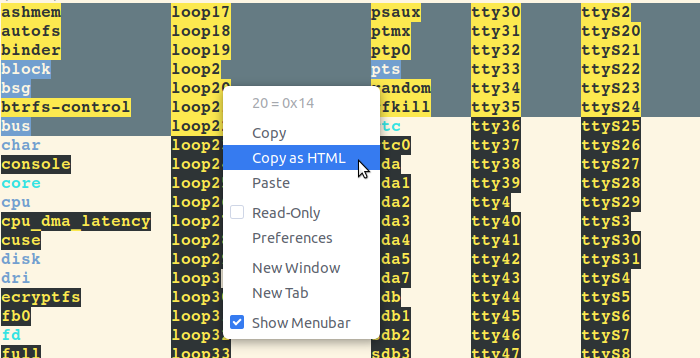
\includegraphics[width=0.5\linewidth]{ubuntu-html}
\caption{Converting terminal output to HTML on Ubuntu 18.04+.}
\label{fig:ubuntu-conv}
\end{figure} 

Generally speaking, one needs to fulfill the following requirements:
\begin{enumerate}
\item Have a way of converting terminal output to HTML.
\item Be able to run the HTML to \LaTeX\ Python \href{https://github.com/xziyue/latex-beautiful-listings-screenshot/blob/master/html2tex_gui.py}{script}. Currently, the script is dependent on \href{https://pypi.org/project/wxPython/}{\rawinline|wxPython|}, \href{https://pypi.org/project/TexSoup/}{\rawinline|TexSoup|} and \href{https://pypi.org/project/PyLaTeX/}{\rawinline|PyLaTeX|}.
\end{enumerate}

To typeset this screenshot in \LaTeX, one needs to run the Python script and paste the HTML in the upper text box. By pressing the ``Convert`` button, the corresponding \LaTeX\ code will appear in the bottom text box, as it is shown in Figure \ref{fig:python-html2latex}. The result is shown as below.

\begin{tcbsrccode}{text}
\input{console-dev.txt}
\end{tcbsrccode}
\input{console-dev.txt}

\begin{figure}[htpb]
\centering
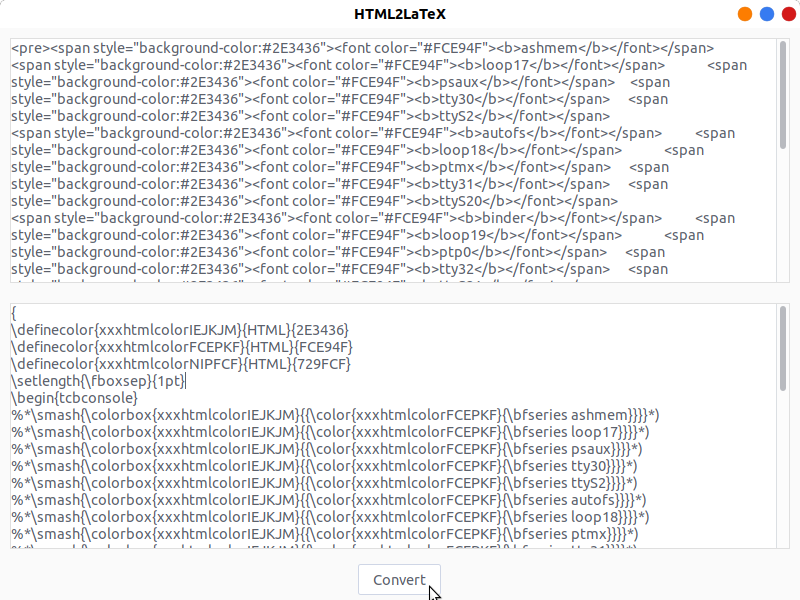
\includegraphics[width=0.5\linewidth]{html2latex}
\caption{Using Python script to convert HTML to \LaTeX.}
\label{fig:python-html2latex}
\end{figure} 

Other classic command-line tools, such as \rawinline|emacs|, are supported as well.

\begin{tcbsrccode}{text}
\input{console-emacs.txt}
\end{tcbsrccode}
\input{console-emacs.txt}


\subsection{Unicode Support}

\section{Add Captions}


\end{document}